\documentclass[12pt,twoside]{article}
\usepackage[dvipsnames]{xcolor}
\usepackage{tikz,graphicx,amsmath,amsfonts,amscd,amssymb,bm,cite,epsfig,epsf,url}
\usepackage[hang,flushmargin]{footmisc}
\usepackage[colorlinks=true,urlcolor=blue,citecolor=blue]{hyperref}
\usepackage{amsthm,multirow,wasysym,appendix}
\usepackage{array,subcaption} 
% \usepackage[small,bf]{caption}
\usepackage{bbm}
\usepackage{pgfplots}
\usetikzlibrary{spy}
\usepgfplotslibrary{external}
\usepgfplotslibrary{fillbetween}
\usetikzlibrary{arrows,automata}
\usepackage{thmtools}
\usepackage{blkarray} 
\usepackage{textcomp}
\usepackage[left=0.8in,right=1.0in,top=1.0in,bottom=1.0in]{geometry}
\usepackage{listings}
%% Probability operators and functions
%
% \def \P{\mathrm{P}}
\def \P{\mathrm{P}}
\def \E{\mathrm{E}}
\def \Var{\mathrm{Var}}
\let\var\Var
\def \Cov {\mathrm{Cov}} \let\cov\Cov
\def \MSE {\mathrm{MSE}} \let\mse\MSE
\def \sgn {\mathrm{sgn}}
\def \R {\mathbb{R}}
\def \C {\mathbb{C}}
\def \N {\mathbb{N}}
\def \Z {\mathbb{Z}}
\def \cV {\mathcal{V}}
\def \cS {\mathcal{S}}

\newcommand{\RR}{\ensuremath{\mathbb{R}}}

\DeclareMathOperator*{\argmin}{arg\,min}
\DeclareMathOperator*{\argmax}{arg\,max}
\newcommand{\red}[1]{\textcolor{red}{#1}}
\newcommand{\blue}[1]{\textcolor{blue}{#1}}
\newcommand{\green}[1]{\textcolor{ForestGreen}{ #1}}
\newcommand{\fuchsia}[1]{\textcolor{RoyalPurple}{ #1}}



%
%% Probability distributions
%
%\def \Bern    {\mathrm{Bern}}
%\def \Binom   {\mathrm{Binom}}
%\def \Exp     {\mathrm{Exp}}
%\def \Geom    {\mathrm{Geom}}
% \def \Norm    {\mathcal{N}}
%\def \Poisson {\mathrm{Poisson}}
%\def \Unif    {\mathrm {U}}
%
\DeclareMathOperator{\Norm}{\mathcal{N}}

\newcommand{\bdb}[1]{\textcolor{red}{#1}}

\newcommand{\ml}[1]{\mathcal{ #1 } }
\newcommand{\wh}[1]{\widehat{ #1 } }
\newcommand{\wt}[1]{\widetilde{ #1 } }
\newcommand{\conj}[1]{\overline{ #1 } }
\newcommand{\rnd}[1]{\tilde{ #1 } }
\newcommand{\rv}[1]{ \rnd{ #1}  }
\newcommand{\rM}{\rnd{ m}  }
\newcommand{\rx}{\rnd{ x}  }
\newcommand{\ry}{\rnd{ y}  }
\newcommand{\rz}{\rnd{ z}  }
\newcommand{\ra}{\rnd{ a}  }
\newcommand{\rb}{\rnd{ b}  }
\newcommand{\rt}{\rnd{ t}  }
\newcommand{\rs}{\rnd{ s}  }


\newcommand{\rpc}{\widetilde{ pc}  }
\newcommand{\rndvec}[1]{\vec{\rnd{#1}}}

\def \cnd {\, | \,}
\def \Id { I }
\def \J {\mathbf{1}\mathbf{1}^T}

\newcommand{\op}[1]{\operatorname{#1}}
\newcommand{\setdef}[2]{ := \keys{ #1 \; | \; #2 } }
\newcommand{\set}[2]{ \keys{ #1 \; | \; #2 } }
\newcommand{\sign}[1]{\op{sign}\left( #1 \right) }
\newcommand{\trace}[1]{\op{tr}\left( #1 \right) }
\newcommand{\tr}[1]{\op{tr}\left( #1 \right) }
\newcommand{\inv}[1]{\left( #1 \right)^{-1} }
\newcommand{\abs}[1]{\left| #1 \right|}
\newcommand{\sabs}[1]{| #1 |}
\newcommand{\keys}[1]{\left\{ #1 \right\}}
\newcommand{\sqbr}[1]{\left[ #1 \right]}
\newcommand{\sbrac}[1]{ ( #1 ) }
\newcommand{\brac}[1]{\left( #1 \right) }
\newcommand{\bbrac}[1]{\big( #1 \big) }
\newcommand{\Bbrac}[1]{\Big( #1 \Big)}
\newcommand{\BBbrac}[1]{\BIG( #1 \Big)}
\newcommand{\MAT}[1]{\begin{bmatrix} #1 \end{bmatrix}}
\newcommand{\sMAT}[1]{\left(\begin{smallmatrix} #1 \end{smallmatrix}\right)}
\newcommand{\sMATn}[1]{\begin{smallmatrix} #1 \end{smallmatrix}}
\newcommand{\PROD}[2]{\left \langle #1, #2\right \rangle}
\newcommand{\PRODs}[2]{\langle #1, #2 \rangle}
\newcommand{\der}[2]{\frac{\text{d}#2}{\text{d}#1}}
\newcommand{\pder}[2]{\frac{\partial#2}{\partial#1}}
\newcommand{\derTwo}[2]{\frac{\text{d}^2#2}{\text{d}#1^2}}
\newcommand{\ceil}[1]{\lceil #1 \rceil}
\newcommand{\Imag}[1]{\op{Im}\brac{ #1 }}
\newcommand{\Real}[1]{\op{Re}\brac{ #1 }}
\newcommand{\norm}[1]{\left|\left| #1 \right|\right| }
\newcommand{\norms}[1]{ \| #1 \|  }
\newcommand{\normProd}[1]{\left|\left| #1 \right|\right| _{\PROD{\cdot}{\cdot}} }
\newcommand{\normTwo}[1]{\left|\left| #1 \right|\right| _{2} }
\newcommand{\normTwos}[1]{ \| #1  \| _{2} }
\newcommand{\normZero}[1]{\left|\left| #1 \right|\right| _{0} }
\newcommand{\normTV}[1]{\left|\left| #1 \right|\right|  _{ \op{TV}  } }% _{\op{c} \ell_1} }
\newcommand{\normOne}[1]{\left|\left| #1 \right|\right| _{1} }
\newcommand{\normOnes}[1]{\| #1 \| _{1} }
\newcommand{\normOneTwo}[1]{\left|\left| #1 \right|\right| _{1,2} }
\newcommand{\normF}[1]{\left|\left| #1 \right|\right| _{\op{F}} }
\newcommand{\normLTwo}[1]{\left|\left| #1 \right|\right| _{\ml{L}_2} }
\newcommand{\normNuc}[1]{\left|\left| #1 \right|\right| _{\ast} }
\newcommand{\normOp}[1]{\left|\left| #1 \right|\right|  }
\newcommand{\normInf}[1]{\left|\left| #1 \right|\right| _{\infty}  }
\newcommand{\proj}[1]{\mathcal{P}_{#1} \, }
\newcommand{\diff}[1]{ \, \text{d}#1 }
\newcommand{\vc}[1]{\boldsymbol{\vec{#1}}}
\newcommand{\rc}[1]{\boldsymbol{#1}}
\newcommand{\vx}{\vec{x}}
\newcommand{\vy}{\vec{y}}
\newcommand{\vz}{\vec{z}}
\newcommand{\vu}{\vec{u}}
\newcommand{\vv}{\vec{v}}
\newcommand{\vb}{\vec{\beta}}
\newcommand{\va}{\vec{\alpha}}
\newcommand{\vaa}{\vec{a}}
\newcommand{\vbb}{\vec{b}}
\newcommand{\vg}{\vec{g}}
\newcommand{\vw}{\vec{w}}
\newcommand{\vh}{\vec{h}}
\newcommand{\vbeta}{\vec{\beta}}
\newcommand{\valpha}{\vec{\alpha}}
\newcommand{\vgamma}{\vec{\gamma}}
\newcommand{\veta}{\vec{\eta}}
\newcommand{\vnu}{\vec{\nu}}
\newcommand{\rw}{\rnd{w}}
\newcommand{\rvnu}{\vc{\nu}}
\newcommand{\rvv}{\rndvec{v}}
\newcommand{\rvw}{\rndvec{w}}
\newcommand{\rvx}{\rndvec{x}}
\newcommand{\rvy}{\rndvec{y}}
\newcommand{\rvz}{\rndvec{z}}
\newcommand{\rvX}{\rndvec{X}}


\newtheorem{theorem}{Theorem}[section]
% \declaretheorem[style=plain,qed=$\square$]{theorem}
\newtheorem{corollary}[theorem]{Corollary}
\newtheorem{definition}[theorem]{Definition}
\newtheorem{lemma}[theorem]{Lemma}
\newtheorem{remark}[theorem]{Remark}
\newtheorem{algorithm}[theorem]{Algorithm}

% \theoremstyle{definition}
%\newtheorem{example}[proof]{Example}
\declaretheorem[style=definition,qed=$\triangle$,sibling=definition]{example}
\declaretheorem[style=definition,qed=$\bigcirc$,sibling=definition]{application}

%
%% Typographic tweaks and miscellaneous
%\newcommand{\sfrac}[2]{\mbox{\small$\displaystyle\frac{#1}{#2}$}}
%\newcommand{\suchthat}{\kern0.1em{:}\kern0.3em}
%\newcommand{\qqquad}{\kern3em}
%\newcommand{\cond}{\,|\,}
%\def\Matlab{\textsc{Matlab}}
%\newcommand{\displayskip}[1]{\abovedisplayskip #1\belowdisplayskip #1}
%\newcommand{\term}[1]{\emph{#1}}
%\renewcommand{\implies}{\;\Rightarrow\;}



\begin{document}

\begin{center}
{\large{\textbf{Homework 2}} } \vspace{0.2cm}\\
Due September 26 at 11 pm
\\
\end{center}

\begin{enumerate}

\item (Geometric random variable)
Let $\ra$ be a geometric random variable with parameter $\alpha$. What is the probability that $\ra$ equals $a$ for $a=1,2,3,\ldots$ if we condition on the event $\ra > 5$? Justify your answer mathematically, and also explain why it makes sense intuitively (for example by referring to the coin flip example that we used to derive the geometric pmf). \\

\subitem
For the random variable $\ra$ to equal $a$ for $a=0,1,2,3,\ldots$ we need to build a geometric distribution with parameter $\alpha$. $\alpha$ will represent the probability of the event happening, (coinflip = heads), and the geometric distribution is the pmf which represents the number of consecutive occurrences of an event before a non-occurrence (i.e. 10 heads before a tails). Therefore, our distribution will follow this formula:
$$ 
   p(\ra) = (\alpha)^a \times (1-\alpha)
$$ 

If we condition on the event $\ra > 5$, then the $p(a)$ for $a \in \{0,1,2,3,4,5\} = 0$. This intuitively makes sense, if we know for a fact we already flipped 6 coins and each of them were heads, our streak of heads could not have possibly ended on the first, second, third, fourth, or fifth flip. \\

On the other hand, if we know we had at least 5 heads in a row, it increases the chance we will have $a>5$ heads drastically. We can condition on the event $a>5$ by using conditional probability to remove the information we know that didn't happen ($a\leq 5$) and then normalize (blow up) the rest of our probability space so the remaining probabilities sum to 1: \\
$$
    P(\ra|a>5) = \frac{(\alpha)^a \times (1-\alpha)}{1-P(a\leq 5)} 
$$

Also, intuitively, the fact that we flipped 5 heads has no influence on the probability of the 6th,7th, or any other coinflip, as they are all independent.  Therefore, I believe that the above statement would be equivalent to the following as well due to independence:
$$
    P(\ra|a>5) = (\alpha)^{a-6} \times (1-\alpha)
$$
Note that the first term in the equation the exponent is adjusted by subtracting 6. That is because we know we have a streak of heads going larger than 5, so we must have made 6 consecutive heads already. The chance our streak ends at 6 is $1-\alpha$ (we flip no more additional heads, and the next coinflip is a tails).

\break


\item (Chess games) Garry and Anish decide to play 10 chess games. Garry wins 4, they draw 4, and Anish wins 2. We decide to model the games probabilistically, assuming that they are independent and in each game Garry has a probability $\theta$ of winning and Anish has a probability $\alpha$ of winning.

\begin{enumerate} 
\item Plot the log-likelihood function of the parametric model.
\subitem We can derive the log-likehood function of our games similarly to how we did in lecture for the Bernoulli distribution. 
$$
    Log-likelyhood \ Function = 2Log(\alpha) + 4Log(\theta) + 4Log(1-\theta - \alpha)
$$
The following is the 3-d plot of the log-likelihood function. \\

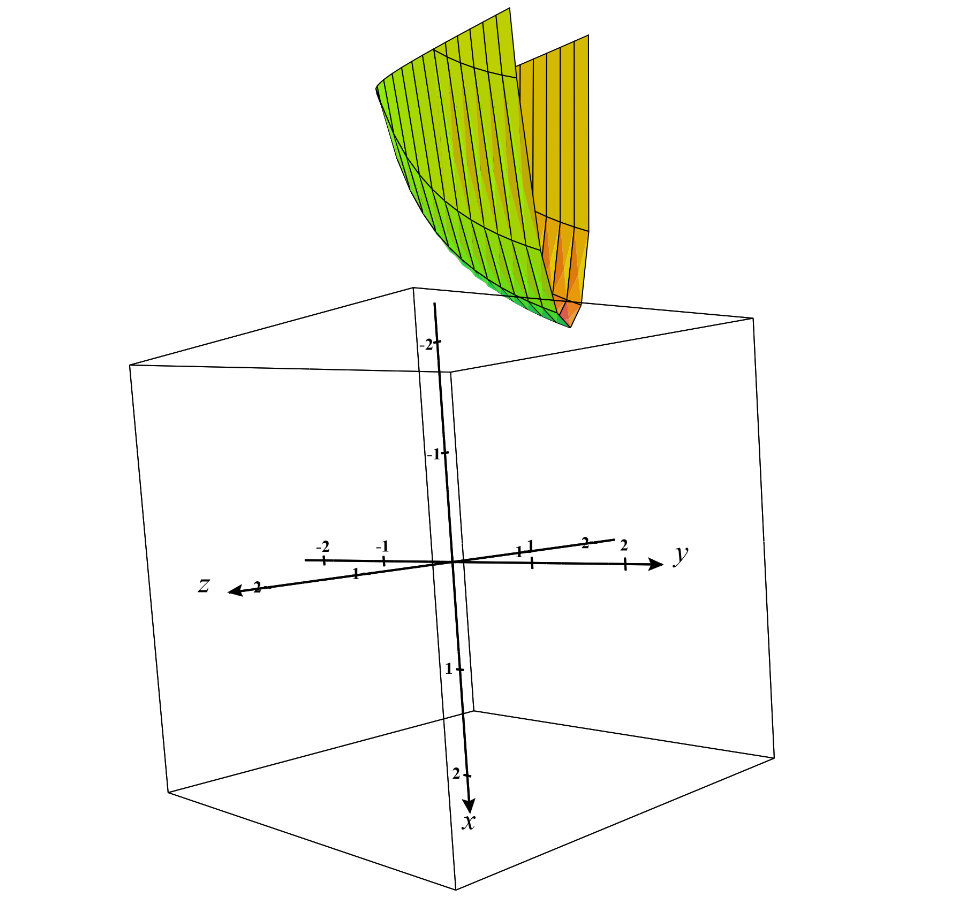
\includegraphics[scale=.5]{hw2 3d plot.png}
\\
It looks ugly. 

\item What is the maximum likelihood estimate of $\theta$ and $\alpha$?
\subitem

After calculating the log likelihood function we can take the derivative and set it to 0. After confirming the point of interest is a global maximum, we find that the maximum likelihood estimate that best models the data is when  $\theta$ is equal to $\frac{\theta}{n}$ and for $alpha$ it would be $\frac{\alpha}{n}$\\

So since Garry won 4 games and Anish won 2 games out of ten total games ($n$) the maximum likehood estimates for $\alpha$ and $\theta$ are $\theta = \frac{4}{10}$ and $\alpha = \frac{2}{10}$

\item Model the data as realizations from a discrete random variable and compute its empirical pmf. Compare this nonparametric model to the parametric model from the previous questions.  
\end{enumerate}
\subitem
If we model the data as realizations from a discrete random variable its computed pmf would be as follows: $$
    p(\theta) = \frac{\text{number of Garry wins}}{\text{total games played}} = \frac{4}{10} \  p(\alpha) = \frac{\text{Number of Annish wins}}{Total Games Played} = \frac{2}{10}$$
    $$
    p(draw) = \frac{\text{Number of draws}}{\text{Total Games Played}} = \frac{4}{10}
$$

The empirical probabilities are the same as the parametric model in part b). This makes sense because when performing MLE, we need to pick parameters that make the data we observed the most probable. Intuitively, the probability that will do so is the empirical probability. 

\item (Darts) In a game of darts, a player needs to hit a certain number $k$ times. Assume that all attempts are mutually independent, and that the probability of success in each attempt is $\theta$. Derive the pmf of a random variable representing the number of required attempts.
\subitem
Here we can model the pmf as very similarly to a binomial distribution pmf, with probability of success as $\theta$ and the probability of failure as $1-\theta$. We need to hit a number of darts $k$ times, so we shoot until we hit our $k$th shot. We shoot a total of $n$ shots, with $n=$ number of misses $+$ number of makes. But, before we write our formula, we must adjust our combinators portion (the binomial coefficient). If we're making our last shot (to arrive at a total of $k$ makes) we don't have n degrees of freedom in our binomial coefficient, but rather, $n-1$, and we choose $k-1$ combinations. Therefore our formula is: 
$$
    p(k)    =  \begin{pmatrix}
    n-1 \\
    k-1
    \end{pmatrix} \times \theta ^k \times (1-\theta)^{n-k}
$$

\break 
\item (Call center)
Complete the code in the iPython notebook: 

\url{https://github.com/cfgranda/prob_stats_for_data_science/blob/main/modeling_discrete_data/call_center_EXERCISE.ipynb}

Verify that you reproduce the figures in the notes (no need to submit them), and submit your code for the functions \emph{empirical\_pmf} and \emph{poisson\_model}.
\subitem
\begin{lstlisting}[language=Python]
#Some code formatting got screwed up when put into LateK
days_in_month = {"January":31,
"February":28,
"March":31,
"April":30,
"May":31,
"June":30,
"July":31,
"August":31,
"September":30,
"October":31,
"November":30,
"December":31}


def empirical_pmf(months, max_count,time_ini,time_end,verbose):
    
    #Create two lits, one to hold extracted data, 
    #other for pmf, and total_calls variable for denominator 
    pmf = list(np.zeros(max_count))
    data = []
    total_call_amount = 0
    
    #Iterate over months
    for month in months:
        
        #Aquire call data for months
        data = compute_counts(time_ini,time_end,month,verbose)
        
        #Iterate over all data points
        for data_point in range(days_in_month[month]):
            #Increment the pmf, i.e. if there were 
            #10 calls on a day, increment index 10 by 1
            #Make sure that it doesnt exceed max count
            if int(data[data_point]) <= max_count-1 and 
                -> is_weekend(month_number, data_point+1) is False:
                pmf[int(data[data_point])] += 1
                
                #Increment the total number of data points
                total_call_amount += 1
            
    
    #Normalize pmf as a probability
    #(divide each element by total_calls)
    for y in range(0,max_count):
        pmf[y] = pmf[y] / total_call_amount
        
    #make pmf a numpy array
    pmf = np.array(pmf)
    
    #Return our pmf -> np.array
    return pmf

def poisson_model(months, max_count,time_ini,time_end,verbose):
    
    #Variables to hold data as its extracted, running total, total observations, and pmf
    data = []
    total_calls = 0
    total_observations = len(months)*max_count
    pmf = list(np.zeros(max_count))
    
    #Extract all data
    for month in months:
        data = compute_counts(time_ini,time_end,month,verbose)
        for i in range(0,max_count):
            #Add all the calls to the total
            total_calls += data[i]
    
    #Calculate lambda -- is this right?
    poi_lambda = total_calls / total_observations
    
    #Define poisson function, forula from wikipedia
    def poisson_function(poi_lambda, periods):
            top_half = (poi_lambda**periods)*(math.e**(-1*poi_lambda))
            bot_half = math.factorial(periods)
           return top_half / bot_half
           
    #Calcualte our pdf
    for x in range(0,max_count):
        pmf[x] = poisson_function(poi_lambda,x)
        
    #make pmf a numpy array
    pmf = np.array(pmf)
    
    #Return our pmf -> np.array
    return pmf
    
\end{lstlisting}



\end{enumerate}
\end{document}
